\documentclass{book}
\usepackage{xcolor}
\usepackage[final]{listings}
\usepackage{graphicx}
\usepackage{hyperref}
\lstloadlanguages{Matlab}
\lstset{language=Matlab}
\author{Bart Vermeulen}
\title{ADCPtools}

\begin{document}
	\maketitle
	\chapter{Getting started}
	\section{Getting help}
	To get an overview of all the functions in adcptools run
	\begin{lstlisting}
		help 
	\end{lstlisting}
	This will display all the avilable functions and clicking on the function name will display the help of the function.

	\section{Vessel mounted ADCP data processing}
	To process vessel mounted ADCP data, it is convenient to store all the collected data files from one deployment into a folder.
	The data can be read with the following line:
	\begin{lstlisting}
		data=readDeployment(depName, path)
	\end{lstlisting}
	in which \lstinline{depName} is the deployment name (i.e. the common part of the files to be read) and \lstinline{path} the folder where the files are located.
	The output is a structure that can contains all the data.

	To check the path sailed by the vessel:
	\begin{lstlisting}
		[x,y]=utmADCP(data);
	      	plot(x,y)
		axis equal
	\end{lstlisting}

	To process repeat transect data, it is necessary to first define which ensembles belong to a specific cross section and and to a certain crossing. This is done using the \lstinline{tid} matrix.
	\begin{figure}
		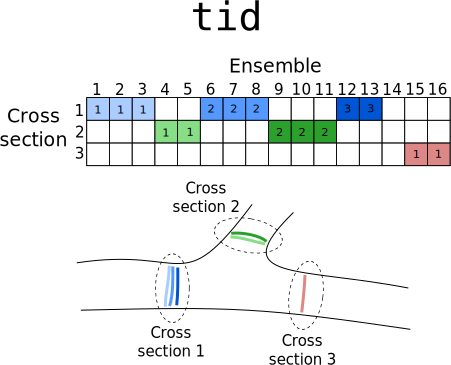
\includegraphics[width=\linewidth]{figures/tid.pdf}
		\caption{Example of a a transect ID matrix. Three cross-section are defined and for each transect different repeat-transect are distinguished. White elements in the matrix indicate zero value.}
		\label{fig:tid}
	\end{figure}
%
%	\chapter{Introduction}
%
%	\chapter{Reading data}
%
%	\chapter{Low level processing}
%
%	\chapter{Transect data processing}
%


%	Repeat transect can be processed with the function \lstinline{proctrans}. 
%
%	\funcdef{msh=procTrans(adcp.tid)}
%	
%	This functions accepts two inputs:
%	\begin{itemize}
%		\item An ADCP structure \verb#adcp# read with \verb#readDeployment.m#.
%		\item A transect ID matrix \verb#tid#. 
%	\end{itemize}
%	\verb#tid# is a matrix of integral numbers with as many columns as ensembles in \verb#adcp# and as many rows as cross-sections you want to process. Any non-zero number at \verb#(i,j)# indicates that the \verb#j#-th ensemble is part of the \verb#i#-th cross-section. The number itself indicates grouping of the ensembles withing a cross-section. If, for example, in one row we have numbers from \verb#1# to \verb#3#, this indicates that all ensembles with number \verb#1# belong together, like all with number \verb#2#, etc. This allows to group subsets of the data within one cross-section (\autoref{fig:tid})
%

%
	\chapter{Coupled ADCP processing}

\end{document}
